\documentclass[pmlr]{jmlr}% new name PMLR (Proceedings of Machine Learning Research)

 % The following packages will be automatically loaded:
 % amsmath, amssymb, natbib, graphicx, url, algorithm2e

 %\usepackage{rotating}% for sideways figures and tables
\usepackage{longtable}% for long tables

 % The booktabs package is used by this sample document
 % (it provides \toprule, \midrule and \bottomrule).
 % Remove the next line if you don't require it.
\usepackage{booktabs}
 % The siunitx package is used by this sample document
 % to align numbers in a column by their decimal point.
 % Remove the next line if you don't require it.
\usepackage[load-configurations=version-1]{siunitx} % newer version
 %\usepackage{siunitx}
 
 % OG from doc https://en.wikibooks.org/wiki/LaTeX/Tables#Floating_with_table 
 \usepackage{multirow}

 % The following command is just for this sample document:
\newcommand{\cs}[1]{\texttt{\char`\\#1}}

 % Define an unnumbered theorem just for this sample document:
\theorembodyfont{\upshape}
\theoremheaderfont{\scshape}
\theorempostheader{:}
\theoremsep{\newline}
\newtheorem*{note}{Note}

 % change the arguments, as appropriate, in the following:
\jmlrvolume{1}
\jmlryear{2010}
\jmlrworkshop{Workshop Title}

\title[SLAPI]{Simultaneous Localization and Active Phenomenon Inference (SLAPI)}

 % Use \Name{Author Name} to specify the name.

 % Spaces are used to separate forenames from the surname so that
 % the surnames can be picked up for the page header and copyright footer.
 
 % If the surname contains spaces, enclose the surname
 % in braces, e.g. \Name{John {Smith Jones}} similarly
 % if the name has a "von" part, e.g \Name{Jane {de Winter}}.
 % If the first letter in the forenames is a diacritic
 % enclose the diacritic in braces, e.g. \Name{{\'E}louise Smith}

 % *** Make sure there's no spurious space before \nametag ***

 % Two authors with the same address
  \author{\Name{Olivier L. Georgeon} \Email{ogeorgeon@univ-catholyon.fr}\\
  \addr UR Confluence, Sciences et Humanités (EA 1598) - Lyon Catholic University, France\\
   \Name{Titouan Knockaert} \Email{titouan.knockaert@gmail.com}\\
  \addr Université Claude Bernard Lyon 1, LIRIS CNRS UMR5205, F-69622 Villeurbanne, France
}

 % Three or more authors with the same address:
 % \author{\Name{Author Name1} \Email{an1@sample.com}\\
 %  \Name{Author Name2} \Email{an2@sample.com}\\
 %  \Name{Author Name3} \Email{an3@sample.com}\\
 %  \Name{Author Name4} \Email{an4@sample.com}\\
 %  \Name{Author Name5} \Email{an5@sample.com}\\
 %  \Name{Author Name6} \Email{an6@sample.com}\\
 %  \Name{Author Name7} \Email{an7@sample.com}\\
 %  \Name{Author Name8} \Email{an8@sample.com}\\
 %  \Name{Author Name9} \Email{an9@sample.com}\\
 %  \Name{Author Name10} \Email{an10@sample.com}\\
 %  \Name{Author Name11} \Email{an11@sample.com}\\
 %  \Name{Author Name12} \Email{an12@sample.com}\\
 %  \Name{Author Name13} \Email{an13@sample.com}\\
 %  \Name{Author Name14} \Email{an14@sample.com}\\
 %  \addr Address}


 % Authors with different addresses:
 % \author{\Name{Author Name1} \Email{abc@sample.com}\\
 % \addr Address 1
 % \AND
 % \Name{Author Name2} \Email{xyz@sample.com}\\
 % \addr Address 2
 %}

\editor{Editor's name}
 % \editors{List of editors' names}

\begin{document}

\maketitle

\begin{abstract}
This is the abstract for this article.
\end{abstract}
\begin{keywords}
List of keywords
\end{keywords}

\section{Introduction}
\label{sec:intro}

The problem of getting mobile robots to autonomously learn the position of surrounding objects, recognize them, and keep track of their relative displacements is considered by many to be a key prerequisite of truly autonomous robots. 
Within this framework, the SLAM problem (Simultaneous Localization and Mapping) has been formalized and studied since the 1990s: constructing and updating a map of an unknown environment while simultaneously keeping track of the robot's position within it \citep[e.g.,][]{taketomi_visual_2017}.
SLAM algorithms are tailored to the available resources: odometric sensors, sensors of the environment, computational capacities, as well as the landmarks' properties, quantity, and dynamics, and the usage intended for the robot.

When displacements are imprecise and odometric data is not available, when landmarks are not directly identifiable, and below a certain level of scarcity and noise in the sensory data relative to the environment’s complexity, it becomes difficult to perform SLAM accurately enough to use the robot for tasks involving complex navigation \citep{gay_towards_2021}. 
For such robots, we propose the SLAPI problem:  Simultaneous Localization and Active Phenomenon Inference.
In contrast with SLAM, SLAPI does not aim at constructing a map to use for navigation. 
Instead, it aims at organizing behavior spatially in the vicinity of objects to design robots that exhibit intrinsic motivation \citep[e.g.,][]{oudeyer_intrinsic_2007} such as playfulness and curiosity as they discover and interact with unknown objects. 
Possible applications may not include delivery tasks but may include entertainment and games, similar to playing with pets. 

SLAPI makes no assumption that landmarks can be directly and passively uniquely identified through sensors. 
The robot must rather actively interact with objects, possibly from different angles and through different modalities of control loops, to categorize and recognize objects, and possibly use them as landmarks. 
We call this process \textit{active phenomenon inference}, drawing from the work of \cite{friston_world_2021} on active inference. 
Here the term \textit{phenomenon} refers to the knowledge of physical objects actively constructed by the robot from its point of view and ``as the robot experiences the object through interaction'' \citep{thorisson_explanation_2021}. 

We designed a proof-of-concept algorithm to illustrate the SLAPI problem. 
We demonstrated it in a robot mounted on omnidirectional wheels and endowed with an echo-localization sensor, photosensitive sensors, and an inertial measurement unit, but no camera and lidar. 
As the robot circles around an object, it constructs the phenomenon corresponding to this object under the form of the set of the spatially-localized control loops that the object affords to the robot. 
New elements can be subsequently added to this set as the robot improves its knowledge of the object. 
Results show that the robot drew out a few cries of amusement and endearment from some human observers, which encourages us to keep improving this range of algorithms. 

Moreover, we believe that the study of SLAPI problems can shed some light on how animals construct knowledge of objects through sensorimotor interactions, while keeping this knowledge grounded in experience. 
It can also provide an angle of attack to the more general AI problem of self-motivated open-ended learning in the real world.

\section{The representational status of sensory data}
\label{sec:input}

An autonomous agent faces the necessity to actively infer the existence and the properties of objects in its environment when the data that it receives through sensors does not already hold a representational correspondence with such objects. 
The representational status of sensory data has been discussed times and again at the philosophical level \citep[e.g.,][]{williford_husserls_2013}.
Loosely, two hypotheses collide: the hypothesis that sensory data carry information about features of the world, versus the hypothesis that sensory data carry information about the agent's experience of interaction with the world. 
We refer to the former as the \textit{representationalist hypothesis}, and to the latter as the \textit{constructivist hypothesis} because it relates to Piaget's theory of construcitivist learning based on sensorimotor schemes \citep{guillermin_artificial_2022}. 

SLAPI falls within the constructivist hypothesis because it applies to robots that have coarse sensors that do not provide much descriptive information about the environment. 
The robot must probe the world a little bit like a blind person who uses a cane to actively construct a mental representation of its surroundings. 
Probing experiences consist of control loops during which the robot interacts with the environment.   
They are triggered by an action intended by the robot and result in an outcome that is informative not of the object itself but of the possibility of interaction afforded by the object to the robot. 
\figureref{fig:cycle} shows this cycle of interaction. 
The agent selects an action associated with spatial information that specify how the control loop should be enacted in the environment. 
In return, the agent receives an outcome associated with spatial information that describe how the control loop has been enacted. 


\begin{figure}[htbp]
	% Caption and label go in the first argument and the figure contents
	% go in the second argument
	\floatconts
	{fig:cycle}
	{\caption{The interaction cycle. Black bullet: the cycle begins with the agent sending an action containing spatial information to enact in the environment (right). Black arrowhead: the cycle ends with the agent receiving the outcome containing spatial information (left).}}
	{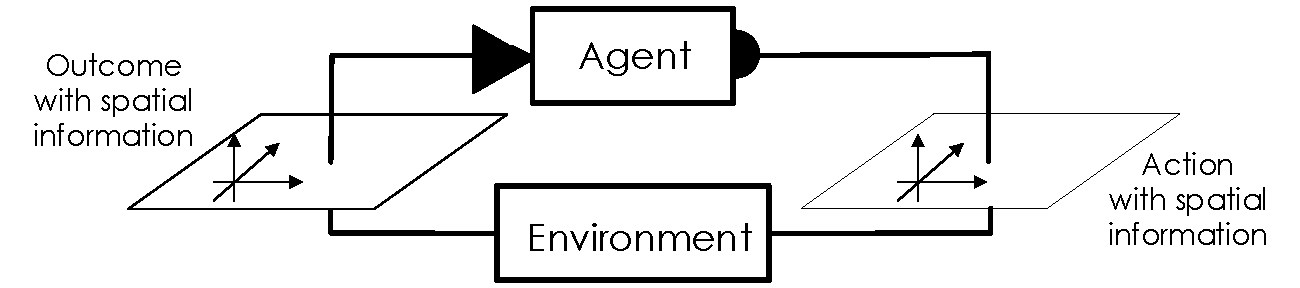
\includegraphics[width=0.8\linewidth]{images/Figure_0_Cycle}}
\end{figure}

Note that this model does not systematically exclude that the outcome carries information about features of the environment. 
We only avoid baking this assumption in the algorithm \textit{a priori}. 
As \cite{rudrauf_mathematical_2017} state about their model based on active inference: ``All we need here is the idea that in one way or another the sensory organs provide an independent source of input and correction for the continually updated world model'' (p. 19).

\section{The experimental setup}
\label{sec:experiment}

We use the robot cat made by Osoyoo\footnote{\url{https://osoyoo.com/2019/11/08/omni-direction-mecanum-wheel-robotic-kit-v1/}}, to which we added an inertial measurement unit.  (\figureref{fig:robot}).

\begin{figure}[htbp]
	% Caption and label go in the first argument and the figure contents
	% go in the second argument
	\floatconts
	{fig:robot}
	{\caption{The robot}}
	{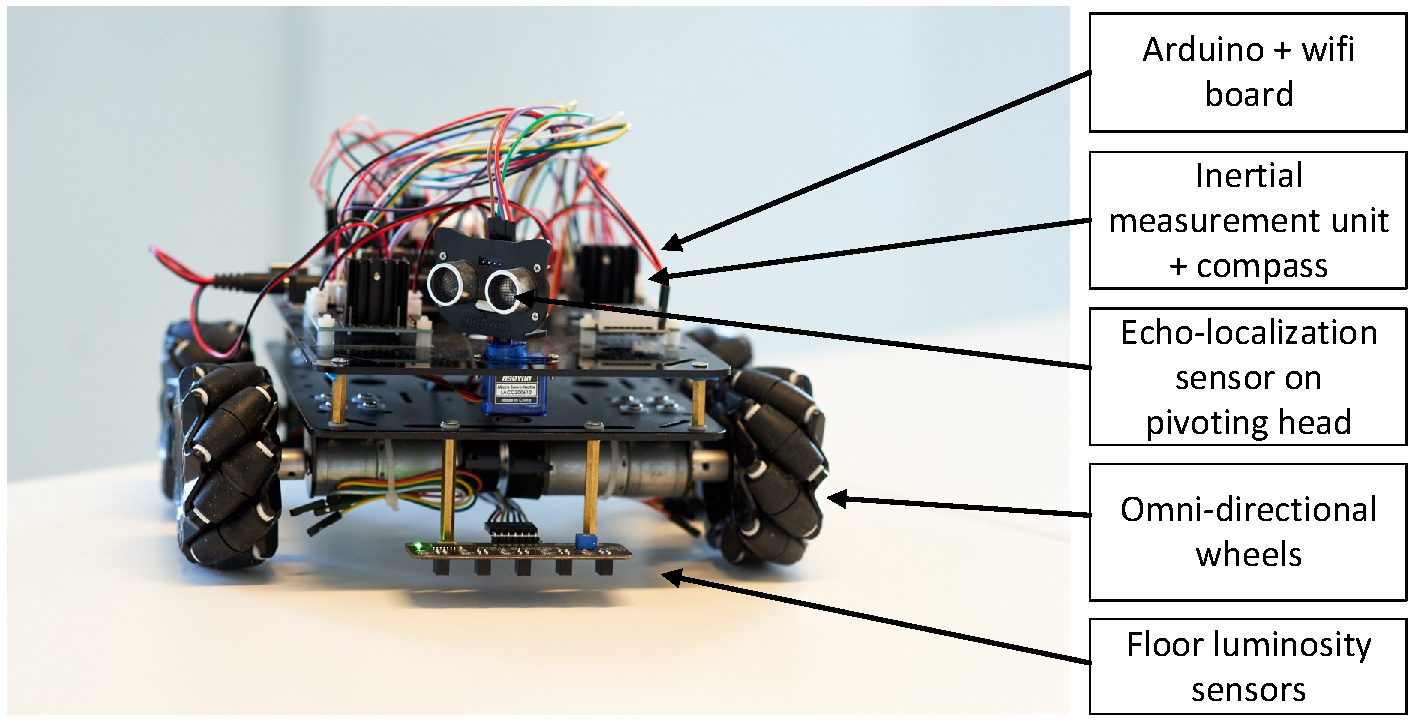
\includegraphics[width=0.8\linewidth]{images/Figure_1_Robot}}
\end{figure}



\section{The software architecture and algorithm}
\label{sec:software}

The data exchanged between the PC and the robot is as follows: 

\begin{altdescription}{PC to Robot}
	\item[PC to Robot] Action code, focus position $(x, y)$, estimated speed $(x,y)$.
	\item[Robot to PC] Outcome code, echo distance, head direction, yaw, azimuth, duration.
\end{altdescription}


\begin{table}[htbp]
	% The first argument is the label.
	% The caption goes in the second argument, and the table contents
	% go in the third argument.
	\floatconts
	{tab:actions}%
	{\caption{Data exchanged between the PC and the robot through wifi}}%
	{\begin{tabular}{l|l}
			\toprule
			PC to Robot & Action code, focus position (x, y), estimated speed (x,y)\\
			\midrule
			Robot to PC & Outcome code, echo distance, head direction, yaw, azimuth, duration\\
			\bottomrule
	\end{tabular}}
\end{table}


\begin{figure}[htbp]
	% Caption and label go in the first argument and the figure contents
	% go in the second argument
	\floatconts
	{fig:architecture}
	{\caption{The software architecture. 
			The \textit{Memory} plays the role of the database, and the \textit{Workspace} plays the role of the Model in a regular Model-View-Controller architecture. 
			The \textit{Workspace} contains the \textit{Synthesizer} which infers the phenomena, and 
			the \textit{Decider} which selects the next intended interaction to send to the robot through wifi (bottom). 
			The \textit{Memory} contains the egocentric memory and the allocentric memory which are accessed through the \textit{Workspace} and the \textit{View Controllers} to display on screen (right).}}
	{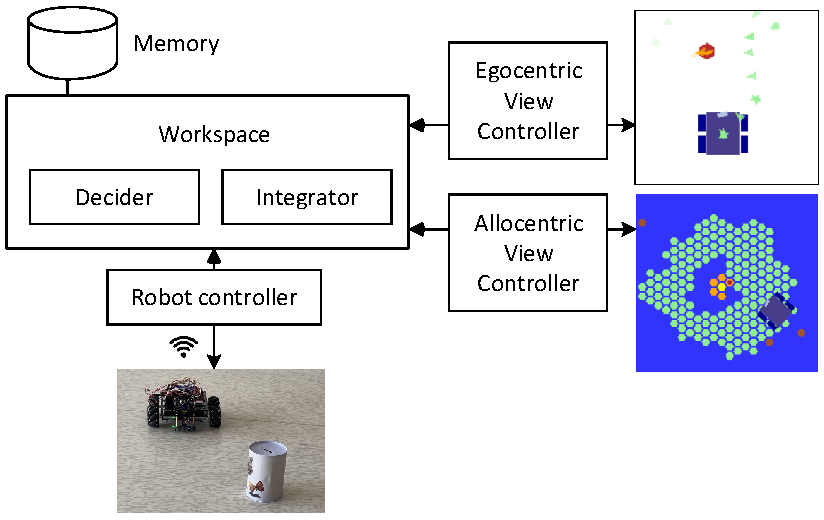
\includegraphics[width=0.8\linewidth]{images/Figure_2_Architecture}}
\end{figure}


\subsection{The actions and outcome}


\begin{table}[htbp]
	\floatconts
	{tab:subtabex}
	{\caption{Actions available to the robot and their possible outcomes}}
	{%
		\subtable[Actions]{%
			\label{tab:ab}%
			\begin{tabular}{lc}
				\toprule
				\bfseries Action & \bfseries Span\\
				\midrule
				Forward & \multirow{4}{3cm}{During 1 second or until line detection}\\
				Backward &  \\
				Shift left &  \\
				Shift right & \\ \hline
				Turn left & $\pi/4$ \\
				Turn right & $-\pi/4$ \\ \hline
				Head scan & $[-\pi/2, \pi/2]$ \\
				\bottomrule
		\end{tabular}}
		\qquad
		\subtable[Outcomes]{%
			\label{tab:cd}%
			\begin{tabular}{lc}
				\toprule
				\bfseries Outcome & \bfseries Description\\
				\midrule
				Line left & \multirow{3}{3cm}{Floor sensors cross luminosity threshold } \\
				Line front & \\
				Line right & \\ \hline
				Echo lost focus & No echo where expected \\ \hline
				Echo left & \multirow{6}{3cm}{Direction and range of the nearest echo}\\  
				Echo right &  \\  
				Echo far left & \\  
				Echo far right & \\  
				Echo far front & \\
				Echo close front & \\ \hline
				Default & No line, no echo \\ 
				\bottomrule
			\end{tabular}
		}
	}
\end{table}


\subsection{The allocentric memory}

The allocentric memory is inspired by the hippocampus in the mammalian brain \citep{grieves_representation_2017}.
We implemented hexagonal cells which can have status as follows: 

\begin{altdescription}{Unknown}
	\item[Unknown] The cell has not yet been inspected.
	\item[Free] The cell affords no interaction.
	\item[occupied] The cell is occupied bu the robot itself.
	\item[Line] A line interaction was enacted here.
	\item[Echo] En echo interaction was enacted here.
\end{altdescription}

\section{Results}

\section{Conclusion}

This example is meant to illustrate a more profound epistemological assumption that the world \textit{in itself} cannot be accessed through direct representational data. This idea goes back to Kant, relates to Piaget's developmental psychology and constructivist epistemology, and has echos in modern physics. 
Kark Friston said that addressing this problem may open the door to the third wave of AI \cite[time code 22:66]{videoFriston}. 



\bibliography{olivier}


\end{document}
